\section{Abstract Data Type} \index{abstract data type} \index{ADT}

\vspace{0.5\parskip}

\begin{definition}[Abstract Data Type]
    An abstract data type (ADT) is a set of mathematical objects and a set of operations on those objects. An ADT describes how information can be used in a program, which is important for specification and provides modularity and reuseability.
\end{definition}

\begin{example}[ADT for Integers]
    \hfill
    \begin{itemize}
        \item Objects: $\Z$
        \item Operations: $\textsc{Add}(x,y)$ $\textsc{Substract}(x,y)$, $\textsc{Multiply}(x,y)$, $\textsc{Quotient}(x,y)$, and \\ $\textsc{Remainder}(x,y)$.
    \end{itemize}
\end{example}
\begin{example}[Stack ADT]
    \hfill
    \begin{itemize}
        \item Objects: sequences
        \item Operations: $\textsc{Push}(S)$ $\textsc{Pop}(S)$, $\textsc{Empty}(S)$.
    \end{itemize}
\end{example}


\section{Data Structures}

\vspace{0.5\parskip}

\begin{definition}[Data Structure] \index{data structure}
    A data structure is an implementation of an abstract data type.
\end{definition}

\begin{example}[Data Structures for Stack]
    A data structure for stacks is an array with a counter. Alternatively, a stack can be implemented as a singly linked list with the top of the stack at the beginning of the list.
\end{example}

An ADT specifies what kind of data you can have and what you can do with the data. A data structure specifies how the data is implemented; in other words, it specifies how the data is stored and how you actually do the operations on the data.

\section{Algorithm Compleixty}

The complexity of an algorithm tells us the amount of resources used by the algorithm, expressed by a function of the size of the input. Such resources can be time, space, number of messages, numbers of bits of communication, etc. We are interested in analyzing the complexity of algorithms because it allows us to:

\begin{itemize}
    \item compare different algorithms
    \item give bound to resources needed for a given input
    \item determine the largest size of input for which the algorithm is still efficient
\end{itemize}

The definition of input size depends on the problem that we are interested in. Below are examples of some common definitions of input size for the type of data that we are dealing with.

\begin{itemize}
    \item integer: number of bits
    \item list: number of elements
    \item array: dimension of the array, or number of bits
    \item graph: number of vertices, or number of edges, or both
\end{itemize}

\section{Dictionary ADT and Implementations}

\subsection{Dictionary ADT}

In this seciton, we will take a look at an example of ADT and some implementation of it. For the dictionary ADT, the objects are defined to be the set of elements each of which has a key drawn from a totally ordered set. And the dictionary ADT should support the following operations:

\begin{itemize}
    \item $\textsc{Search}(S,k)$: search the set $S$ for an element with the key $k$ and return a pointer to one such element. If no such element exists, return $\textsc{nil}$.
    \item $\textsc{Insert}(S,x)$: insert element pointed by the pointer $x$ into the set $S$.
    \item $\textsc{Delte}(S,x)$: delete the element pointed to by the pointer $x$ from the set $S$.
\end{itemize}

Each element $x$ will contain a property $k$ that stores the key.

\begin{remark}
    Some examples of totally ordered sets are: $\Z$, $\Q$, $\R$, colors, English words. The set of complex numbers $\mathbb{C}$ is not totally ordered. A more formal definition of a total order can be found in the notes on Theory of Computation (CSC 240/CSC 236).
\end{remark}

\subsection{Data Structures for Dictionary}

There are many ways to implement a dictionary. The simplest and most common way is to use a hash table, but there are also equally valid implementations.

\subsubsection{Hashing}

$\textsc{Search}$: average complexity $O(1)$, worst-case complexity $O(n)$ \\
$\textsc{Insert}$: average complexity $O(1)$, worst-case complexity $O(n)$ \\
$\textsc{Delete}$: average complexity $O(1)$, worst-case complexity $O(n)$

\subsubsection{Array}

We can use two arrays, one with keys, the other with values in the correesponding position of the keys. In the case of unsorted arrays, the time complexities of the operations are:

$\textsc{Search}$: worst-case complexity $O(n)$; since unsorted, we need to perform linear search to find the element \\
$\textsc{Insert}$: worst-case complexity $O(1)$ \\
$\textsc{Delete}$: worst-case complexity $O(1)$

Another assumption that we need to make is that the elements and keys are placed consecutively in the array. However, empty slots might be created upon deleting elements. To solve this, we simply replace the deleted element with the last element in the array. By doing so, we ensure that the number of elements in $S$ is at most the size of the array.

\subsubsection{Binary Search Tree}

$\textsc{Search}$: $\Theta(h)$
$\textsc{Insert}$: $\Theta(h)$ \\
$\textsc{Delete}$: $\Theta(h)$ \\
where $h$ is the height of the tree.

\subsubsection{Sorted Array with Counter}

$\textsc{Search}$: $O(\log n)$ using binary search \\
$\textsc{Insert}$: $\Theta(n)$ \\
$\textsc{Delete}$: $\Theta(n)$

\subsubsection{Unsorted Singly Linked List}

$\textsc{Search}$: $\Theta(n)$ \\
$\textsc{Insert}$: $\Theta(1)$ \\
$\textsc{Delete}$: $\Theta(n)$; this is because for a singly linked list, it takes $\Theta(n)$ time to find the pointer to the previous element in order to reconnect the links after deleting

\subsubsection{Unsorted Doubly Linked List}

$\textsc{Search}$: $\Theta(n)$ \\
$\textsc{Insert}$: $\Theta(1)$ \\
$\textsc{Delete}$: $\Theta(1)$

\subsubsection{Sorted Doubly Linked List}

$\textsc{Search}$: $\Theta(n)$; we cannot perform binary search because we don't know the length of the array \\
$\textsc{Insert}$: $\Theta(n)$ to insert into the correct position to keep the list sorted \\
$\textsc{Delete}$: $\Theta(1)$

\subsubsection{Direct Access Table} \index{direct access table}

If our set of keys $S$ is a subset of some finite universe $U = \{ 0, 1, \ldots, m-1 \}$ where $|U| = m$, then we can use a direct access table to implement a dictionary ADT. To represent the dictionary, we use an array $A$ with $m$ slots indexed from 0 to $m$, each of which corresponds to a key in $S$. The value of the slot $A[i]$ is the pointer to the element in the set $S$ with the key $i$. The limitations of such implementation include:

\begin{itemize}
    \item keys have to be unique
    \item size of the list can get arbitrarily large
    \item size of the list is limited
\end{itemize}

\begin{figure}[htbp]
    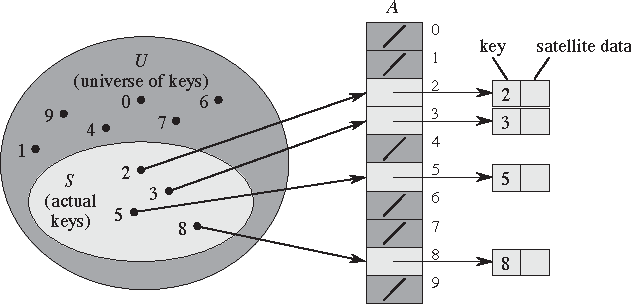
\includegraphics[width=0.6\linewidth]{direct_access_table.pdf}
    \caption{Direct access table}
    \label{fig:direct_access_table}
\end{figure}

\begin{figure}[htbp]
    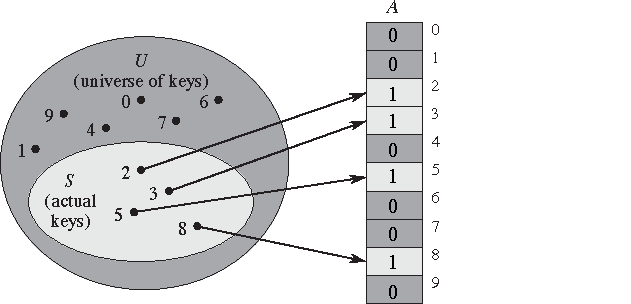
\includegraphics[width=0.6\linewidth]{bitvector_direct_access_table.pdf}
    \caption{Bit vector direct access table}
    \label{fig:bitvector_direct_access_table}
\end{figure}

\begin{codebox}
    \Procname{$\proc{Search}(A,k)$}
    \li $\Return$ $A[k]$
\end{codebox}

\begin{codebox}
    \Procname{$\proc{Insert}(A,x)$}
    \li $A[x.key] = x$
\end{codebox}

\begin{codebox}
    \Procname{$\proc{Delete}(A,x)$}
    \li $A[x.key] = \textsc{nil}$
\end{codebox}

Each of the three operations above takes constant time $O(1)$.

Alternatively, we can use value $1$ to indicate the presence of element at a given slot, and value $0$ to denote the absence of element at a given slot. The resulting data structure called a bit vector direct access table. \index{bit vector direct access table}